\begin{acknowledgementsCH}
 這裡將簡單介紹如何利用\LaTeX\ 來編輯你的畢業論文,若不知道\LaTeX\ 是什麼或是沒有概念的話,建議你可以簡單看過放在此資料夾裡的\href{run:./latex123.pdf}{李果正-大家來學\LaTeX}前四章內容,在下載適合的\LaTeX\ 整合發行套件之後(請看第~\ref{it:download}項),可以嘗試用剛安裝好的\LaTeX\ 編輯器來編譯\href{run:./thesis.tex}{thesis.tex}這份文件,編譯的方法可以看下面第~\ref{it:comp}項的介紹,若編譯成功,所編譯出來的thesis.pdf文件的應該會跟此demo.pdf文件一模一樣,而且沒有任何問號符號,走到這一步的話,就差不多可以開始邊學習\LaTeX\ 邊編輯你的畢業論文了!基本上會使用到的指令都包含在論文的的各章節裡,怎麼在論文裡寫公式或是放圖之類的就自行看tex檔學吧。如果有任何問題或建議可以來信與我討論,我的信箱是\href{mailto:dran31545@gmail.com}{dran31545@gmail.com},或是到此範本\href{http://code.google.com/p/ntu-thesis-latex-template/}{Google Project}裡面的\href{http://code.google.com/p/ntu-thesis-latex-template/issues/list}{Issues}貼上你的問題與建議,我會盡我所能更新此範本,也歡迎大家自行重製、改良此範本並散布給他人,祝大家順利畢業!\\\\
 要編輯致謝請打開\href{run:./acknowledgementsCH.tex}{acknowledgementsCH.tex}\\
 \begin{enumerate}[leftmargin=0pt, topsep=0pt, itemsep=0pt, label=\Roman{*}.]
\item 此範本參考並修改自下列網站的資料:
\begin{enumerate}[topsep=0pt, itemsep=0pt, label=$\bullet$]
    \item \href{http://www.csie.ntu.edu.tw/~tzhuan/www/resources/ntu/}{如何用 LaTeX 排版臺灣大學碩士論文}\\
    \textemdash 台灣大學論文\LaTeX\ 樣版原創者\href{http://www.csie.ntu.edu.tw/~tzhuan/www/}{黃子桓}的教學網頁
    \item \href{http://www.hitripod.com/blog/2012/05/latex-thesis-template-quick-reference/}{LaTeX 常用語法及論文範本}\\
    \textemdash \href{http://www.hitripod.com/blog/}{Hitripod}所修改的範本,這裡參考了許多他所寫的格式和內容
    \item \href{http://www.cc.ntu.edu.tw/chinese/epaper/0014/20100920_1404.htm}{使用LaTeX做出精美的論文}
    \item \href{http://www.hitripod.com/blog/2011/04/xetex-chinese-font-cjk-latex/}{XeTeX:解決 LaTeX 惱人的中文字型問題}
    \item \href{http://code.google.com/p/ntuthesis/}{台灣大學碩士、博士論文的Latex模板}\\
\end{enumerate}
\item 幾個有用的參考資料及網路資源:
\begin{enumerate}[topsep=0pt, itemsep=0pt, label=$\bullet$]
    \item \href{run:./latex123.pdf}{李果正-大家來學\LaTeX}\textemdash 建議先看完前四章
    \item \href{http://en.wikibooks.org/wiki/LaTeX}{WIKIBOOKS-\LaTeX}\textemdash 好用的線上工具書
    \item \href{run:./Working_with_a_bib_file_using_Jabref.pdf}{Working with a .bib file using JabRef}
    \item \href{run:./Fi087_S.pdf}{Using BibDesk - A short tutorial}
    \item \href{http://www.dfcd.net/articles/latex/latex.html}{LaTeX for Physicists}\\
\end{enumerate}
\item 下載\LaTeX\ 整合發行套件,可參考\href{http://www.tug.org/texcollection/}{TeX Collection}:\label{it:download}
 \begin{enumerate}[topsep=0pt, itemsep=0pt, label=\arabic{*}.]
     \item \href{http://www.tug.org/mactex/}{MacTeX}: For \textcolor{Green}{\textbf{MacOSX}},下載\href{http://mirror.ctan.org/systems/mac/mactex/MacTeX.pkg}{MacTeX.pkg}
     \item \href{http://www.tug.org/protext/}{ProTeXt}: For \textcolor{Green}{\textbf{Windows}},下載\href{ftp://ftp.fernuni-hagen.de/pub/windows/win32/ProTeXt/}{ISO file}
     \item \href{http://www.tug.org/texlive/}{TeX Live}: For \textcolor{Green}{\textbf{GNU/Linux}} and \textcolor{Green}{\textbf{MacOSX}}, and \textcolor{Green}{\textbf{Windows}},下載\href{http://www.tug.org/texlive/acquire-iso.html}{ISO file}
     \item \href{http://ctan.org/}{CTAN}: The Comprehensive TeX Archive Network.\\
 \end{enumerate}

\item 好用的程式:
 \begin{enumerate}[topsep=0pt, itemsep=0pt, label=$\bullet$]
    \item 文獻管理系統:
        \begin{enumerate}[topsep=0pt, itemsep=0pt, label=\arabic{*}.]
         \item \href{http://jabref.sourceforge.net/}{JabRef}\\
                     可參考\href{run:./Working_with_a_bib_file_using_Jabref.pdf}{Working with a .bib file using JabRef}或是\href{https://www.google.com/search?q=jabref}{Google}及\href{http://www.youtube.com/results?search_query=jabref}{YouTube}
         \item \href{http://bibdesk.sourceforge.net/}{BibDesk} (For Mac)\\
                     可參考\href{run:./Fi087_S.pdf}{Using BibDesk - A short tutorial}或是\href{https://www.google.com/search?q=bibdesk}{Google}及\href{http://www.youtube.com/results?search_query=bibdesk}{YouTube}
         \end{enumerate}
         \item 方程式編輯器:\href{https://chrome.google.com/webstore/detail/dinfmiceliiomokeofbocegmacmagjhe?hl=zh-TW}{Daum Equation Editor} (Chrome App,必須使用Google瀏覽器)\\
 \end{enumerate} 
\item 編譯流程:\label{it:comp}
\begin{enumerate}[topsep=0pt, itemsep=0pt, label=\arabic{*}.]
    \item \texttt{xelatex thesis}\\ 對thesis.tex進行第一次XeLaTeX編譯,產生thesis.pdf以其他檔案
    \item \texttt{bibtex thesis}\\ 對thesis.tex進行BibTeX編譯,產生bbl檔以及blg檔
    \item \texttt{xelatex thesis}\\ 對thesis.tex進行第二次XeLaTeX編譯,產生目錄、圖表連結及參考文獻
    \item \texttt{xelatex thesis}\\ 對thesis.tex進行第三次XeLaTeX編譯,產生參考文獻連結,完成編譯
\end{enumerate} 
    \textcolor{Red}{注意!}此範本使用cite套件,可依據你利用文獻管理系統所整理好的\href{run:./thesisbib.bib}{thesisbib.bib}檔在論文最後產生參考文獻頁面,若你的系所規定要在每個章節的後面產生參考文獻,則可以用chapterbib套件,來對每個有附參考文獻的章節tex檔進行一次BibTeX編譯產生bbl檔,如範例的\href{run:./introduction.tex}{introduction.tex}、\href{run:./THM.tex}{THM.tex}和\href{run:./EXP.tex}{EXP.tex},如果有這需要請把\href{run:./thesis.tex}{thesis.tex}檔裡使用cite套件的指令利用註解符號\texttt{\%}來取消使用cite套件,並刪去出現在使用chapterbib套件指令前面的註解符號\texttt{\%}來啟動使用chapterbib套件
    \begin{verbatim}
\usepackage{cite}
%\usepackage{chapterbib}
改成
%\usepackage{cite}
\usepackage{chapterbib}
    \end{verbatim}
    再來利用註解符號\texttt{\%}取消會把參考文獻放在論文最後的指令
    \begin{verbatim}
\bibliographystyle{unsrt}
\addcontentsline{toc}{chapter}{\bibname}
\bibliography{thesisbib}
改成
%\bibliographystyle{unsrt}
%\addcontentsline{toc}{chapter}{\bibname}
%\bibliography{thesisbib}
    \end{verbatim}
    再把用來輸入章節檔案的\texttt{\textbackslash input}指令改成\texttt{\textbackslash include}指令
     \begin{verbatim}
\chapter{Introduction}
\label{c:intro}

Attention plays an important role in human vision. For example, when
we look at an image, our eye movements comprise a succession of {\em
fixations} (repetitive positioning of eyes to parts of the image)
and {\em saccades} (rapid eye jump). Those parts of the image that
cause eye fixations and capture primary attention are called {\em
regions of interest} (ROIs). Studies in visual attention and eye
movement have shown that humans generally only attend to a few ROIs.
Detecting these visually attentive regions in images is challenging
but useful in many multimedia applications, such as automatic
thumbnail cropping, object recognition, content-based image
retrieval, adaptive image compression and automatic browsing in
small-screen devices.

Many algorithms have been proposed for automatic ROI detection in
images. Unfortunately, these methods were often evaluated only on
specific and small data sets that are not publicly available. The
lack of published {\em benchmarks} makes experiments non-repeatable
and quantitative evaluation difficult. However, as recommended by
the latest ACM SIGMM retreat, repeatable experiments using published
benchmarks are important for advancing the multimedia research
field~\cite{Rowe:2005:ASR}.

\begin{figure}
\centering
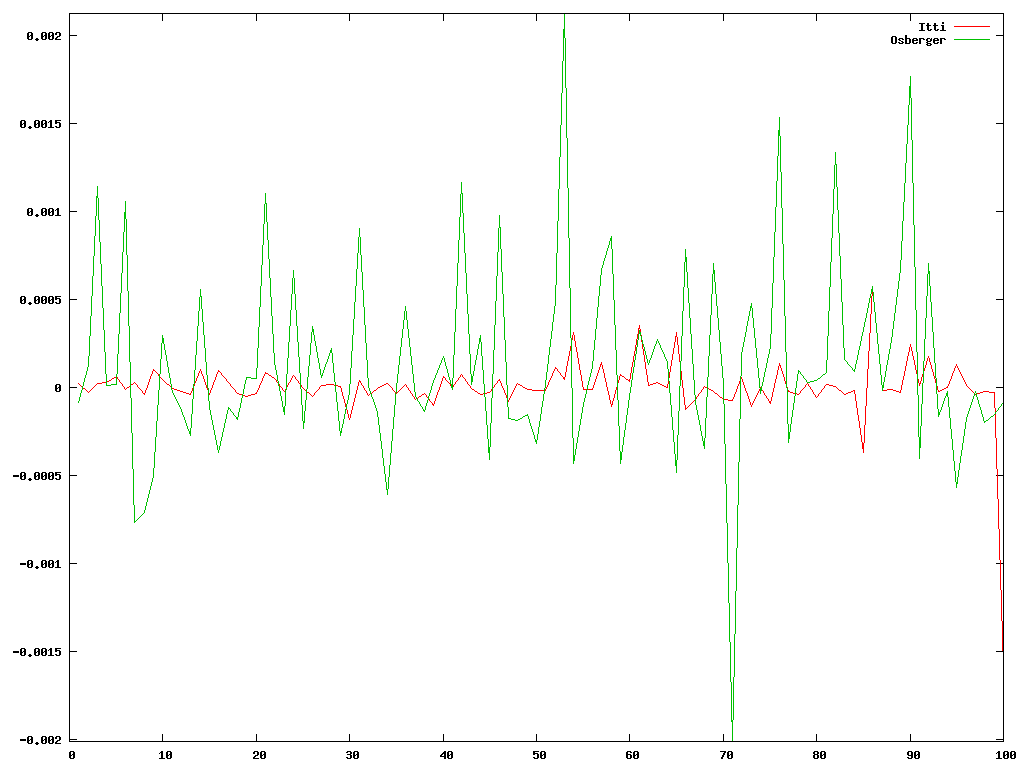
\includegraphics[width=0.45\textwidth]{pics/kl.png}
\caption{kl-distance}
\label{kl}
\end{figure}

\begin{table}[t]
\begin{center}
\begin{tabular}{lcc}

\hline
                    &  {\small Itti's method}     & {\small Fuzzy growing}    \\
\hline
{\small Precision}           &  0.4475    & 0.4506 \\
{\small Recall}              &  0.5515    & 0.5542 \\
\hline

\end{tabular}
\caption[Evaluation of FOA sets]{\small Evaluation of FOA sets. } \label{t:FOA}
\end{center}
\end{table}
  =>  \chapter{Introduction}
\label{c:intro}

Attention plays an important role in human vision. For example, when
we look at an image, our eye movements comprise a succession of {\em
fixations} (repetitive positioning of eyes to parts of the image)
and {\em saccades} (rapid eye jump). Those parts of the image that
cause eye fixations and capture primary attention are called {\em
regions of interest} (ROIs). Studies in visual attention and eye
movement have shown that humans generally only attend to a few ROIs.
Detecting these visually attentive regions in images is challenging
but useful in many multimedia applications, such as automatic
thumbnail cropping, object recognition, content-based image
retrieval, adaptive image compression and automatic browsing in
small-screen devices.

Many algorithms have been proposed for automatic ROI detection in
images. Unfortunately, these methods were often evaluated only on
specific and small data sets that are not publicly available. The
lack of published {\em benchmarks} makes experiments non-repeatable
and quantitative evaluation difficult. However, as recommended by
the latest ACM SIGMM retreat, repeatable experiments using published
benchmarks are important for advancing the multimedia research
field~\cite{Rowe:2005:ASR}.

\begin{figure}
\centering
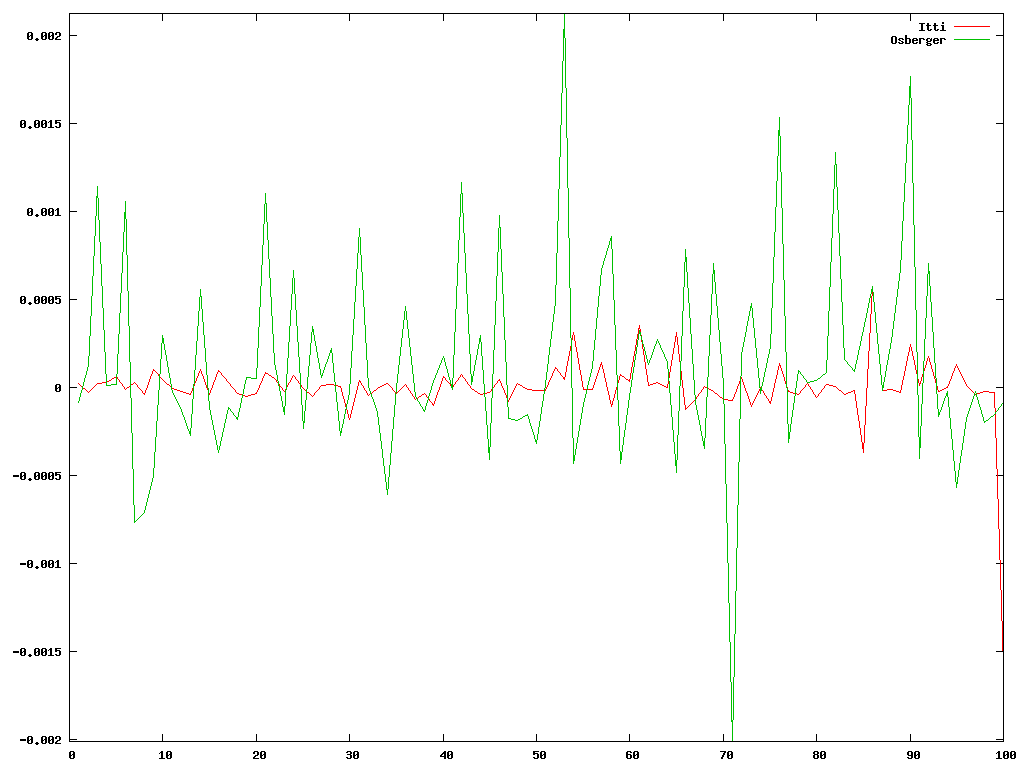
\includegraphics[width=0.45\textwidth]{pics/kl.png}
\caption{kl-distance}
\label{kl}
\end{figure}

\begin{table}[t]
\begin{center}
\begin{tabular}{lcc}

\hline
                    &  {\small Itti's method}     & {\small Fuzzy growing}    \\
\hline
{\small Precision}           &  0.4475    & 0.4506 \\
{\small Recall}              &  0.5515    & 0.5542 \\
\hline

\end{tabular}
\caption[Evaluation of FOA sets]{\small Evaluation of FOA sets. } \label{t:FOA}
\end{center}
\end{table}

\input{THM}           =>  \include{THM}
\input{EXP}           =>  \include{EXP}
     \end{verbatim}
    最後記得在每個有附參考文獻的章節加上產生參考文獻的指令,即在\href{run:./introduction.tex}{introduction.tex}、\href{run:./THM.tex}{THM.tex}和\href{run:./EXP.tex}{EXP.tex}三個檔案裡最後啟動下面兩行指令
     \begin{verbatim}
%\bibliographystyle{unsrt} => \bibliographystyle{unsrt}
%\bibliography{thesisbib}  =>  \bibliography{thesisbib}
     \end{verbatim}
    而編譯時則需要對有附參考文獻的\href{run:./introduction.tex}{introduction.tex}、\href{run:./THM.tex}{THM.tex}和\href{run:./EXP.tex}{EXP.tex}各做一次BibTeX 編譯,編譯流程如下
    \begin{enumerate}[topsep=0pt, itemsep=0pt, label=\arabic{*}.]
    \item \texttt{xelatex thesis}\\ 對thesis.tex進行第一次XeLaTeX編譯,產生thesis.pdf及其他檔案
    \item \texttt{bibtex introduction}\\ 對introduction.tex進行BibTeX編譯,產生bbl檔以及blg檔
    \item \texttt{bibtex THM}\\ 對THM.tex進行BibTeX編譯,產生bbl檔以及blg檔
    \item \texttt{bibtex EXP}\\ 對EXP.tex進行BibTeX編譯,產生bbl檔以及blg檔
    \item \texttt{xelatex thesis}\\ 對thesis.tex進行第二次XeLaTeX編譯,產生目錄、圖表連結及參考文獻
    \item \texttt{xelatex thesis}\\ 對thesis.tex進行第三次XeLaTeX編譯,產生參考文獻連結,完成編譯\\
\end{enumerate} 
\item 補充說明與注意事項:
\begin{enumerate}[topsep=0pt, itemsep=0pt, label=$\bullet$]
    \item 口試委員會審定書:\\
    請到台大圖書館網頁的\href{http://etds.lib.ntu.edu.tw/etdsystem/submit/submitLogin}{電子論文服務}下載\href{http://gra103.aca.ntu.edu.tw/gra2007/gra/tienn/\%E5\%AD\%B8\%E4\%BD\%8D\%E8\%80\%83\%E8\%A9\%A6\%E8\%A1\%A8\%E5\%86\%8A/THESISSAMPLE.DOC}{論文格式範本},並修改成正確的格式,也可到此範本所在資料夾的\href{run:./cert.doc}{cert.doc}修改。當然你也可以利用LaTeX來編輯,你只要填好\href{run:./ntuvars.tex}{ntuvars.tex}檔的資料,並去除在thesis.tex裡下面這行的註解符號\texttt{\%} 
    \begin{verbatim}
%\makecertification
    \end{verbatim}
    編譯完後就可以產生審定書格式。口試通過後,請把已經簽名的審定書掃描成pdf檔,再取代原本的\href{run:./cert.pdf}{cert.pdf},即可放上已簽名的審定書。處理審定書出現的指令在thesis.tex裡 
    \begin{verbatim}
%----------- generate the certification ...
%\makecertification
%----------- includepdf by using package ...
\addcontentsline{toc}{chapter}{口試委員會審定書}
\includepdf[pages={1}]{cert.pdf}
    \end{verbatim}
    \item 浮水印:\\
    資料夾已經附上浮水印檔案了,若學校有更改,到請到台大圖書館網頁的\href{http://etds.lib.ntu.edu.tw/etdsystem/submit/submitLogin}{電子論文服務}下載\href{http://etds.lib.ntu.edu.tw/files/watermark.pdf}{pdf格式的浮水印}到此範本所在資料夾。若要開啟關閉浮水印功能,即自行刪去或加上下面位於\href{run:./thesis.tex}{thesis.tex}指令的註解符號\texttt{\%}
    \begin{verbatim}
%\CenterWallPaper{0.174}{watermark.pdf}
%\setlength{\wpXoffset}{6.1725cm}
%\setlength{\wpYoffset}{10.5225cm}
    \end{verbatim}
    \item 單面印刷與雙面印刷:\\
    此範本為單面印刷,若論文頁數超過80頁,依規定需要用雙面印刷,此時只需把thesis.tex裡的
    \begin{verbatim}
\documentclass[a4paper, 12pt, oneside]{book}
改成
\documentclass[a4paper, 12pt, twoside]{book}
    \end{verbatim}
        \item 如何加入附錄?\\
    在\href{run:./thesis.tex}{thesis.tex}裡,依需求選擇input或include,刪去\texttt{\%}符號來輸入附錄章節
    \begin{verbatim}
%----------- Input your appendix here  -----------
%\chapter{First appendix title}

Open and edit \href{run:./AppendixA.tex}{AppendixA.tex}
%or %chapter cite  == \include
%\chapter{First appendix title}

Open and edit \href{run:./AppendixA.tex}{AppendixA.tex}
    \end{verbatim}
    在章節檔\texttt{AppendixA.tex}裡,開頭打
    \begin{verbatim}
\chapter{First appendix title}
    \end{verbatim}
    即可,以此類推。    
        \item 系上規定論文圖表須全部放到最後獨立出來的章節,且章節不出現在目錄中:\\
    在\href{run:./thesis.tex}{thesis.tex}裡,依需求選擇input或include,刪去\texttt{\%}符號來輸入圖表章節
    \begin{verbatim}    
%----------- Input your Figure chapter here  -----------
%\input{EndFigTab} 
%chapter cite  == \include
%\include{EndFigTab}
    \end{verbatim}
    在章節檔\href{run:./EndFigTab.tex}{EndFigTab.tex}裡有範例和說明可供參考,要注意正文的圖表和附錄的圖表要分清楚,即在\href{run:./EndFigTab.tex}{EndFigTab.tex}內
    \begin{verbatim}    
\renewcommand{\thefigure}{\arabic{chapter}.\arabic{figure}} 
\renewcommand{\thetable}{\arabic{chapter}.\arabic{table}} 
%--- Input your main figures and tables here  ---
    \end{verbatim}
    這幾行之後章節計數器格式已切換為1\dots 9,放正文的圖表 ,
     \begin{verbatim}    
\renewcommand{\thefigure}{\Alph{chapter}.\arabic{figure}} 
\renewcommand{\thetable}{\Alph{chapter}.\arabic{table}}
%--- Input your appendix figures and tables here  ---
    \end{verbatim}
    這幾行之後章節計數器格式已切換為A\dots Z,放附錄的圖表。另外要取消圖表的浮動功能,才能讓圖表按照指令出現順序排好,即把平常使用的圖表指令
    \begin{verbatim}    
\begin{figure}[htb]
...
\begin{table}[htb]
    \end{verbatim}
    改成
     \begin{verbatim}    
\begin{figure}[!]
...
\begin{table}[!]
    \end{verbatim}
    剩下的只要注意章節圖表的計數器設定即可。\texttt{\textbackslash ref}和\texttt{\textbackslash label}指令可以在此圖表章節與正文章節使用。
     \item 如果我想要修改margin(文字邊界)的話,可以從哪裡下手呢?\\
     請打開\href{run:./ntu.sty}{ntu.sty}修改下面這行的上下左右參數即可:
    \begin{verbatim}
\RequirePackage[top=3cm,left=3cm,bottom=2cm,right=3cm]{geometry}
    \end{verbatim}
    \item 我想引用Twomey (1974): Pollution and planetary albedo這篇論文,如何用\texttt{\textbackslash cite}引用它的時候在內文顯示Twomey (1974) [編號] ?\\
    建議使用natbib套件,參考資料如下:\\
    \href{http://en.wikibooks.org/wiki/LaTeX/Bibliography_Management}{LaTeX/Bibliography Management}\\
    \href{http://nodonn.tipido.net/bibstyle.php}{Overview of Bibtex-Styles}\\
    \href{http://merkel.zoneo.net/Latex/natbib.php}{Reference sheet for natbib usage }\
 \item \XeTeX\ :\\
    此範本中文字體使用\XeTeX\ 轉換,細節請參考\href{http://www.hitripod.com/blog/}{Hitripod}寫的\href{http://www.hitripod.com/blog/2011/04/xetex-chinese-font-cjk-latex/}{ 
XeTeX:解決 LaTeX 惱人的中文字型問題}。
 \item 如何輸入英文`單引號'和``雙引號''以及不同長度的破折號?\\
        可以參考\href{run:./latex123.pdf}{李果正-大家來學\LaTeX}第17頁針對標點符號的遊戲規則,範例如下,輸入以下指令:\\
        \begin{verbatim}
`單引號'\\
``雙引號''\\
-hyphen\\
--en-dash\\
---em-dash\\
        \end{verbatim} 
        則顯示:\\
       `單引號'\\
        ``雙引號''\\
        -hyphen\\
        --en-dash\\
        ---em-dash\\
    \end{enumerate} 
    \end{enumerate} 
               

%----------- Have a fractal fern? -----------
%\begin{pspicture}
%\psFern[scale=30,maxIter=100000,linecolor=Green]
%\end{pspicture}

 \end{acknowledgementsCH}